\documentclass{beamer}
\usepackage{hyperref}
\usepackage{url}
\usepackage{natbib}
\usepackage{xcolor}
\usepackage{graphicx}
% \usepackage{tikz}
%\usetheme{vub} 
\usetheme[coloredtitles]{vub}
% \usetheme[showsection]{vub}
\title{Visual Step-By-Step Explanations of Constraint Satisfaction Problems}
\subtitle{ZebraTutor - Explaining logic grid puzzles}
\author{Emilio Gamba\textsuperscript{1}, Bart Bogaerts\textsuperscript{2}, Tias Guns\textsuperscript{1}\\ 
\tiny{\textsuperscript{1}data-lab, Vrije Universiteit Brussel}\\
\tiny{\textsuperscript{2}AI lab, Vrije Universiteit Brussel}\\
\tiny{\{firstname.lastname\}@vub.be}}
\date{}


\newcommand{\phantomgraphics}[2][]{%
  \leavevmode\phantom{\includegraphics[#1]{#2}}%
}


\begin{document}

% Automatic titlepage with VUB logo.
\frame{\maketitle}

%a
\begin{frame}{\small{Explainable Artificial Intelligence (XAI)}}
    \framesubtitle{Motivation}
    \vspace{2cm}
    \textbf{Curse of performance}
    \begin{itemize}
        \item Black-box prediction systems (e.g. deep neural networks)
        \item Efficient complex reasoning systems with millions of parameters
    \end{itemize}

    \begin{figure}[]
        \centering
        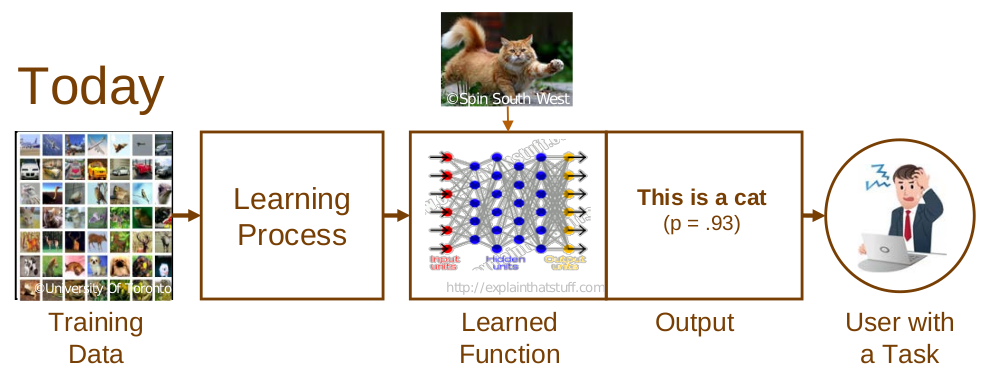
\includegraphics[width=0.8\textwidth]{figures/cat}
        {\small \caption{Deep neural network - image classifier \textsuperscript{\cite{gunning2017explainable}}}}
        \label{catdog}
    \end{figure}

\end{frame}

\begin{frame}{\small{Explainable Artificial Intelligence (XAI)}}
    \framesubtitle{Motivation}

    \vspace{2cm}

    \begin{block}{Human-interpretability}
        \emph{Users should be able to \textbf{see} but also \textbf{study} and \textbf{understand} how inputs are mathematically mapped to outputs.} \textsuperscript{\cite{doran2017does}}
    \end{block}
    \vfill
    \textbf{The A.R.T of Responsible AI \textsuperscript{\cite{adadi2018peeking}}}
    \begin{itemize}
        \item \textbf{\underline{A}ccountability} \textit{need to explain and justify actions to user}
        \item \textbf{\underline{R}esponsibility} \textit{role of answering for one's decisions and identify errors or unexpected results}
        \item \textbf{\underline{T}ransparency} \textit{need to describe, inspect reproduce AI thought process}
    \end{itemize}

\end{frame}

\begin{frame}{\small{Explainable Artificial Intelligence (XAI)}}
    \framesubtitle{Definition}
    \vspace{1cm}
    \vfill

    \begin{center}
        \emph{``XAI is an explanatory agent revealing underlying \textbf{causes} to its or another agent’s decision making''} \textsuperscript{\citep{miller2019explanation}}
    \end{center}
    \begin{flushright}
        --- Miller, 2019
    \end{flushright}
    \vfill

\end{frame}

\begin{frame}{\small{Explaining Constraint Satisfaction Problems}}
    \framesubtitle{Goal : Explainable agency}
    \vspace{2cm}
    Given \emph{objectives} and \emph{background knowledge} relevant to objectives:
    \begin{itemize}
        \item \small{Produce \emph{records of decision} taken during plan generation}
        \item \small{Produce summary of agent's \emph{mental effort}}
        \item \small{Produce \emph{understandable explanations} about specific choices and reasons for them}
    \end{itemize}
    \vspace*{1em}
    \begin{figure}[]
        \centering
        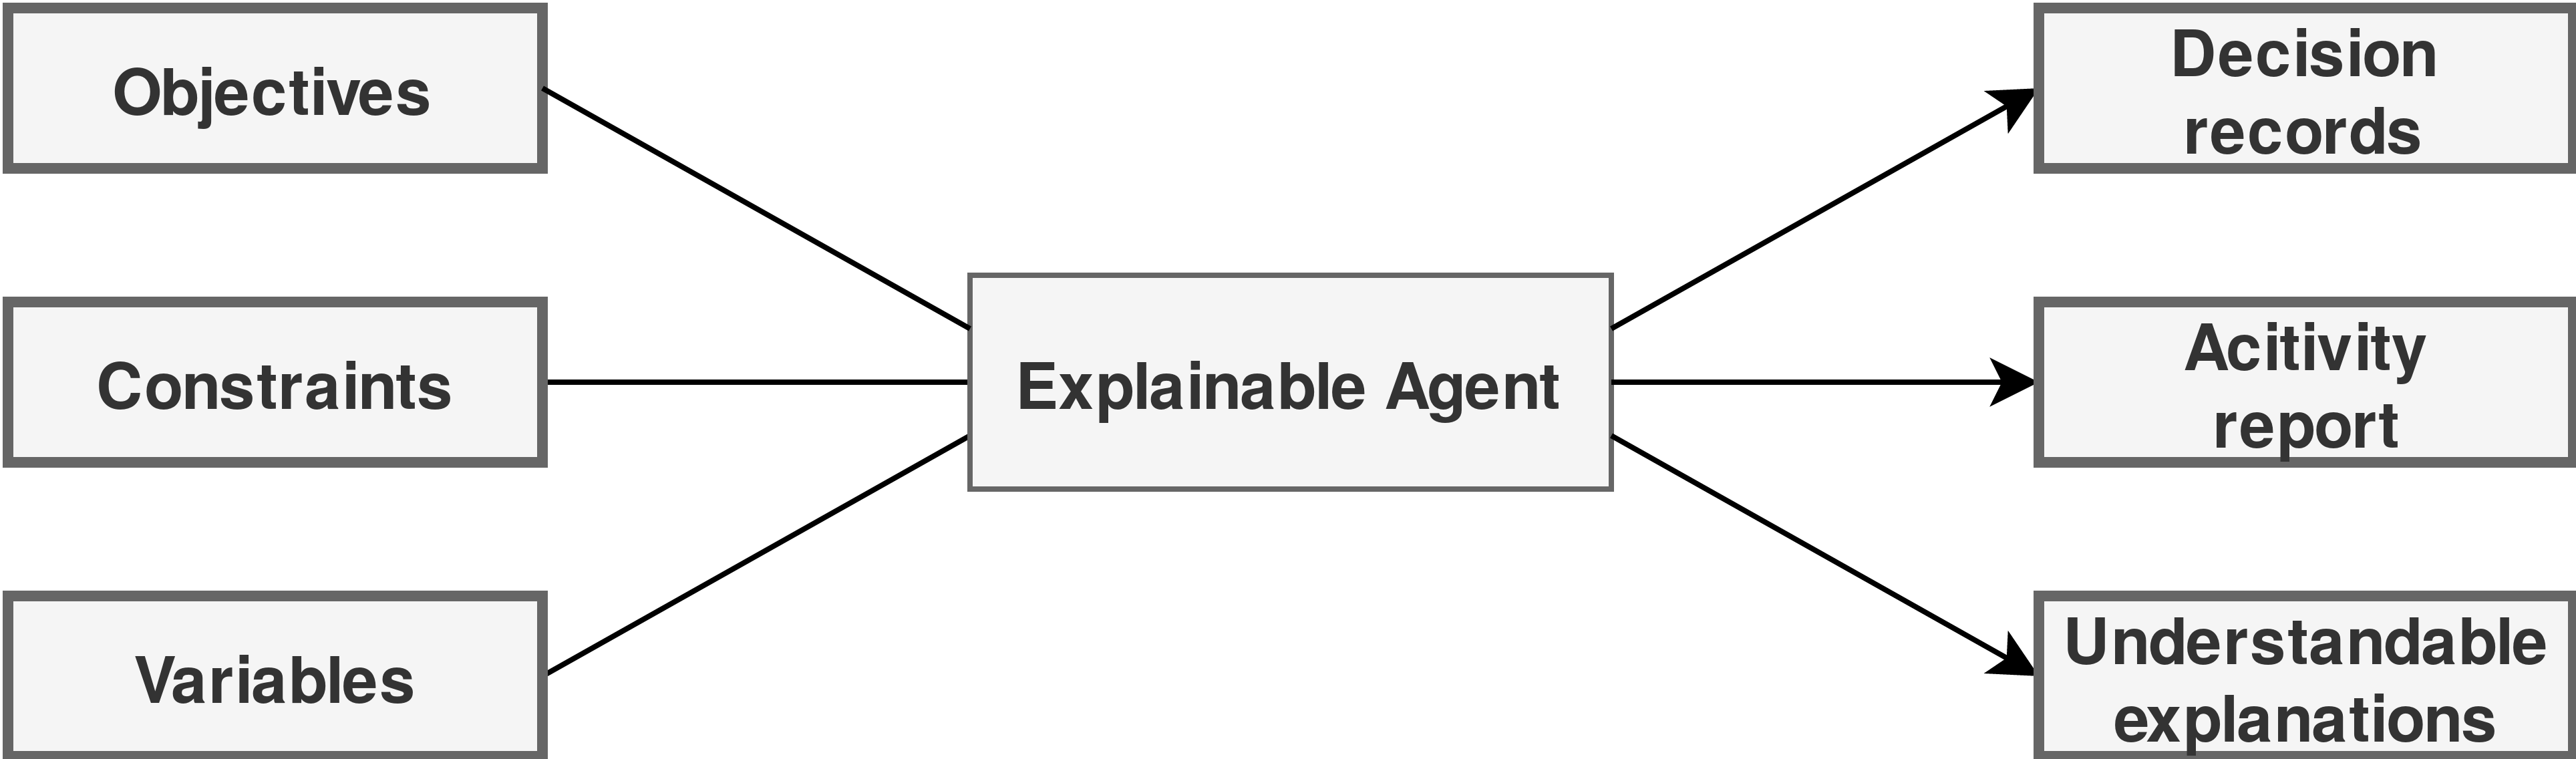
\includegraphics[width=0.8\textwidth]{figures/explainable_agency2}
    \end{figure}


\end{frame}


\begin{frame}{\small{Explaining Constraint Satisfaction Problems}}
    \framesubtitle{ZebraTutor : an \emph{explainable} agent }
    \vspace{1.85cm}


    \only<1>{
        \begin{block}{Problem statement}
            Given the natural language problem statement and set of clues (entities, constraints)
        \end{block}
        \vfill
        \begin{figure}[]
            \centering
            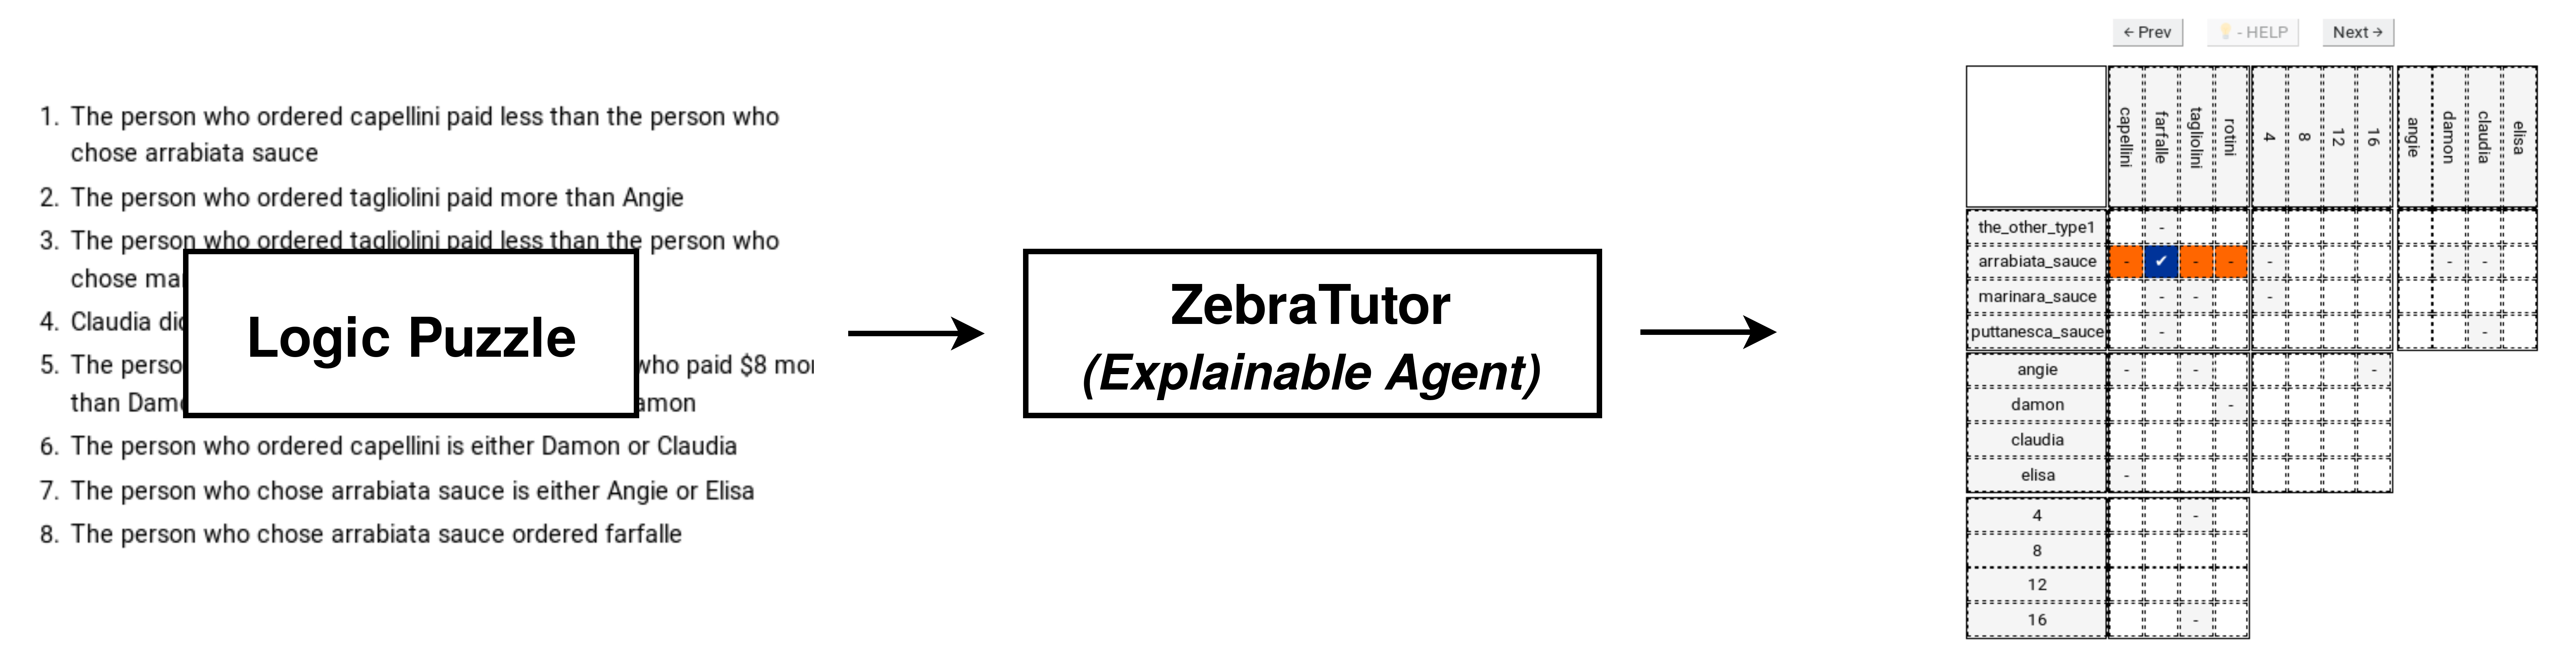
\includegraphics[width=\textwidth]{figures/puzzle_pipeline}
        \end{figure}
    }
    \pause
    \only<2>{
        \begin{block}{Problem statement}
            Given the natural language problem statement and set of clues (entities, constraints):
            \begin{itemize}
                \item Produce the \emph{explanation sequence} to solve the puzzle
                \phantom{\parbox{\linewidth}{\item Produce the cost (mental effort) associated to each step}}
                \phantom{\parbox{\linewidth}{\item Produce the \emph{cognitively-easiest explanation} for each step in the explanation sequence}}
            \end{itemize}
        \end{block}
        \begin{figure}[]
            \centering
            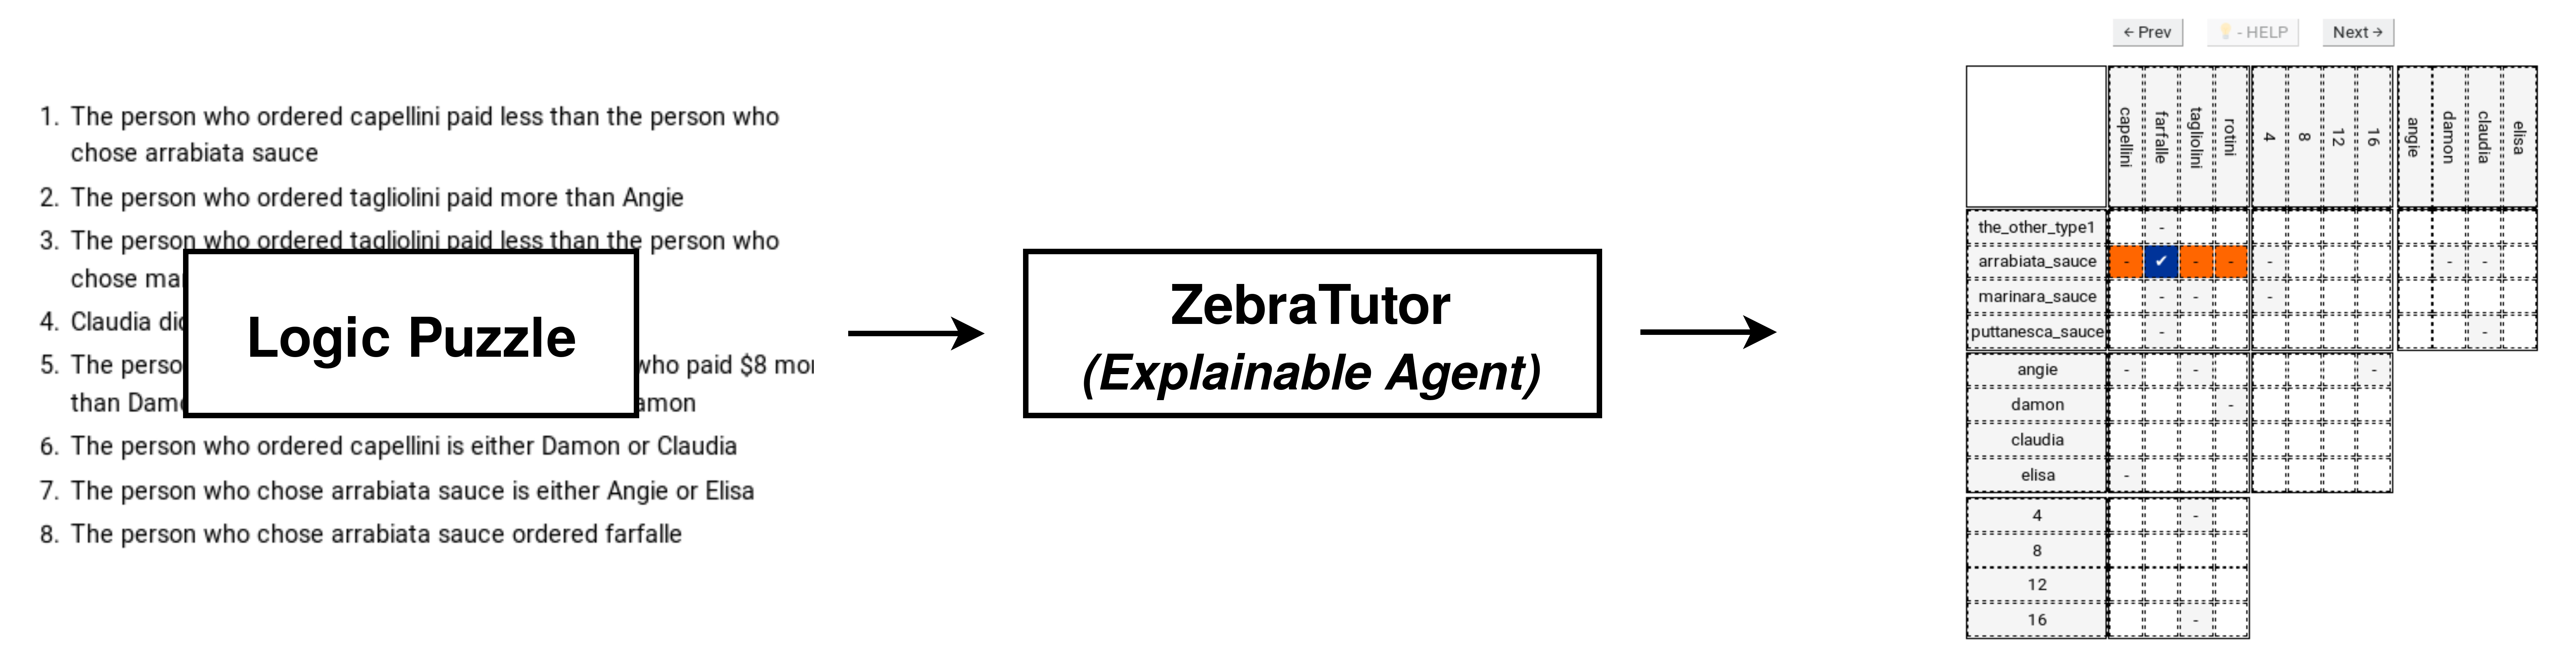
\includegraphics[width=0.8\textwidth]{figures/puzzle_pipeline}
        \end{figure}
    }

    \pause
    \only<3>{
        \begin{block}{Problem statement}
            Given the natural language problem statement and set of clues (entities, constraints):
            \begin{itemize}
                \item Produce the \emph{explanation sequence} to solve the puzzle
                \item Produce the cost (mental effort) associated to each step
                \phantom{\parbox{\linewidth}{\item Produce the \emph{cognitively-easiest explanation} for each step in the explanation sequence}}
            \end{itemize}
        \end{block}
        \begin{figure}[]
            \centering
            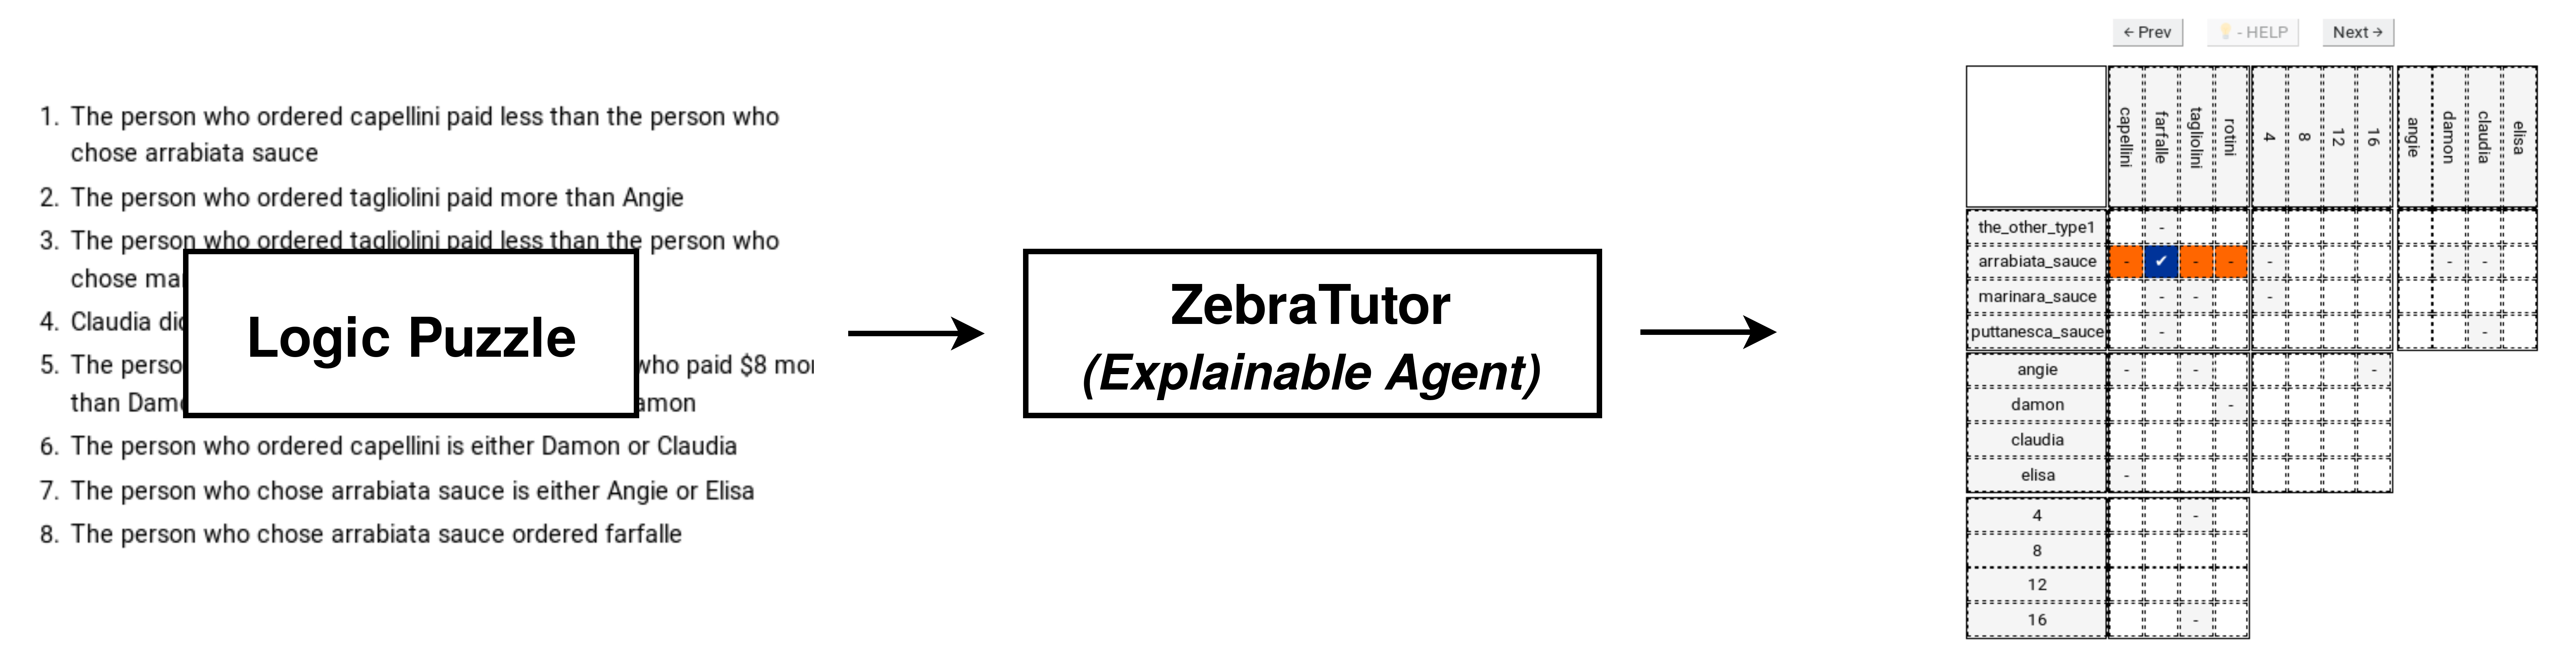
\includegraphics[width=0.8\textwidth]{figures/puzzle_pipeline}
        \end{figure}
    }

    \pause
    \only<4>{
        \begin{block}{Problem statement}
            Given the natural language problem statement and set of clues (entities, constraints):
            \begin{itemize}
                \item Produce the \emph{explanation sequence} to solve the puzzle
                \item Produce the cost (mental effort) associated to each step
                \item Produce the \emph{cognitively-easiest explanation} for each step in the explanation sequence
            \end{itemize}
        \end{block}
        \begin{figure}[]
            \centering
            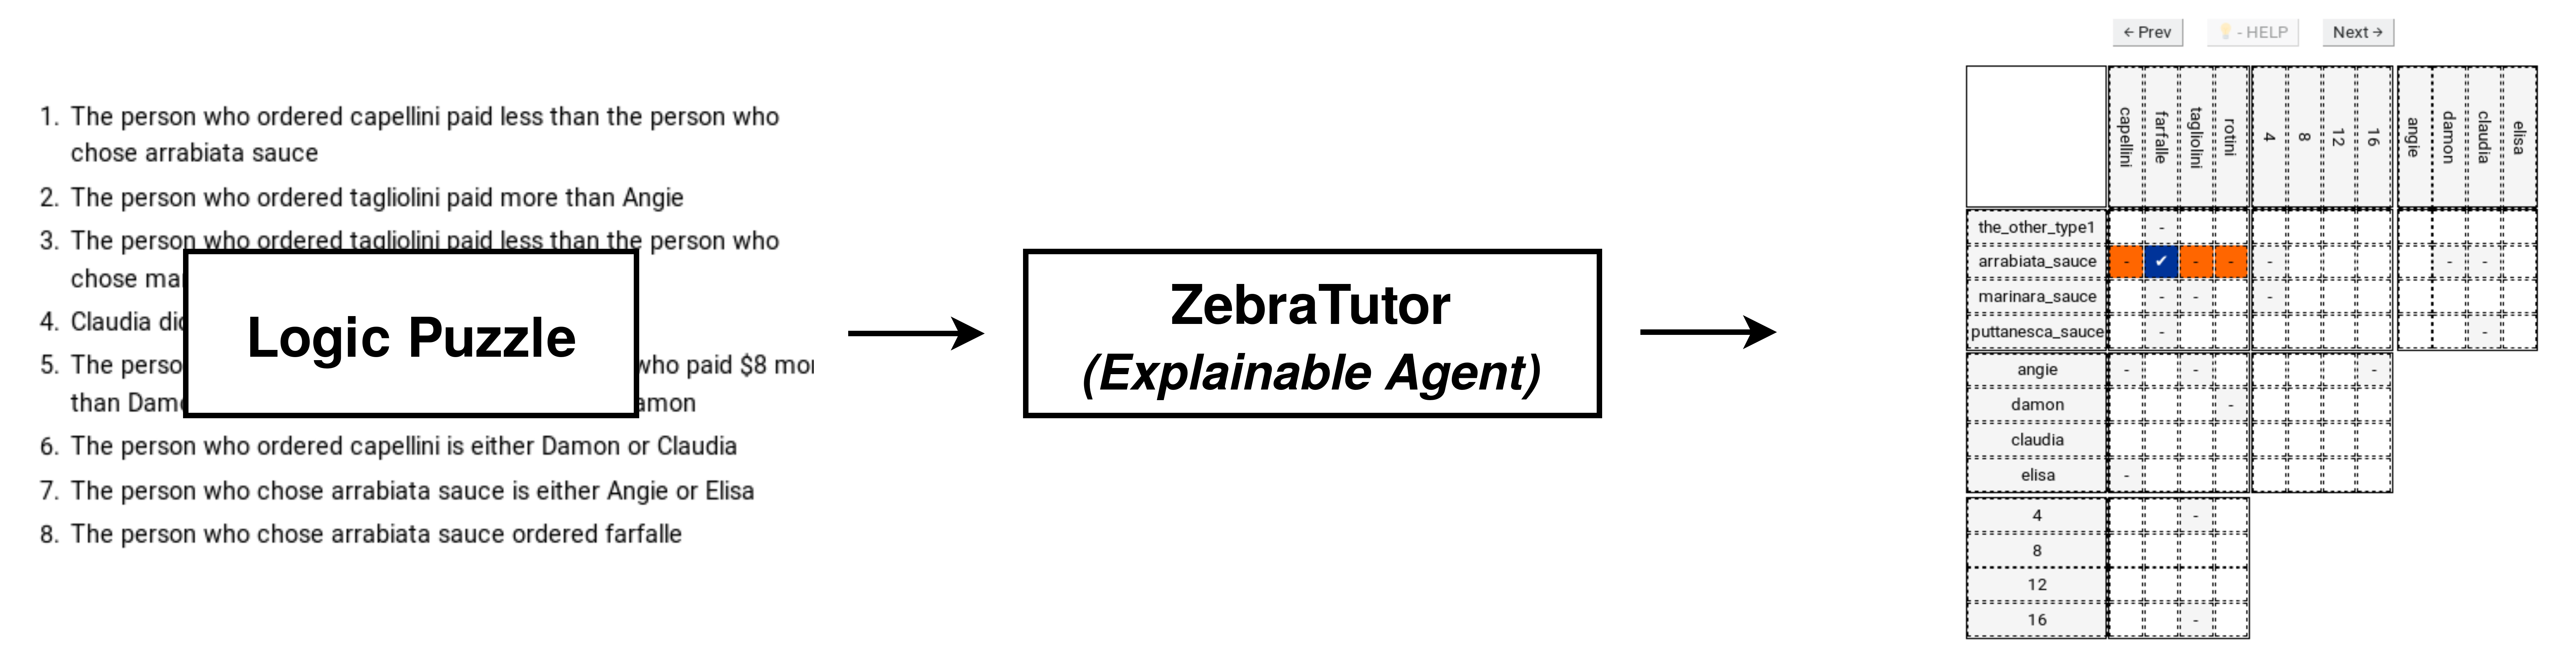
\includegraphics[width=0.8\textwidth]{figures/puzzle_pipeline}
        \end{figure}
    }

    % \vfill


\end{frame}

\begin{frame}{\small{Explaining Constraint Satisfaction Problems}}
    \framesubtitle{ZebraTutor : an \emph{explainable} agent }
    \vspace{1cm}
    % \only<1>{
    %     \begin{block}{Problem statement}
    %         Given the natural language problem statement and set of clues (entities, constraints):
    %         \begin{itemize}
    %             \item Produce the \emph{explanation sequence} to solve the puzzle
    %             \item Produce the cost (mental effort) associated to each step
    %             \item Produce the \emph{cognitively-easiest explanation} for each step in the explanation sequence
    %         \end{itemize}
    %     \end{block}
    %     \phantomgraphics[width=\textwidth]{figures/step_1}%
    % }
    % \only<8>{

    % }
    % \vfill
    % \pause
    \only<1-8>{
        \begin{block}{\textcolor{lightgray}{Problem statement}}
            \textcolor{lightgray}{
                Given the natural language problem statement and set of clues (entities, constraints):}
            \begin{itemize}
                \item \textcolor{lightgray}{Produce the \textcolor{black}{\emph{explanation sequence}} to solve the puzzle}
                \item \textcolor{lightgray}{Produce the cost (\textcolor{black}{mental effort}) \textcolor{black}{associated to each step}}
                \item \textcolor{lightgray}{Produce the \textcolor{black}{\emph{cognitively-easiest explanation}} for each step in the explanation sequence}
            \end{itemize}
        \end{block}
    }
    \only<1>{\begin{figure}[]
            \centering
            
\includegraphics[width=\textwidth]{figures/step_1}
        \end{figure}}
    \pause
    \only<2>{\begin{figure}[]
            \centering
            
\includegraphics[width=\textwidth]{figures/step_2}
        \end{figure}}
    \pause
    \only<3>{\begin{figure}[]
            \centering
            
\includegraphics[width=\textwidth]{figures/step_3}
        \end{figure}}
    \pause
    \only<4>{\begin{figure}[]
            \centering
            
\includegraphics[width=\textwidth]{figures/step_4}
        \end{figure}}
    \pause
    \only<5>{\begin{figure}[]
            \centering
            
\includegraphics[width=\textwidth]{figures/step_5}
        \end{figure}}
    \pause
    \only<6>{\begin{figure}[]
            \centering
            
\includegraphics[width=\textwidth]{figures/step_6}
        \end{figure}}
    \pause
    \only<7>{\begin{figure}[]
            \centering
            
\includegraphics[width=\textwidth]{figures/step_7}
        \end{figure}}
    \pause
    \only<8>{

        \begin{figure}[]
            \centering
            
\includegraphics[width=\textwidth]{figures/step_8}
        \end{figure}}

\end{frame}

\bibliographystyle{abbrv}
\begin{frame}[t,allowframebreaks]
    \frametitle{References}
    \vspace{2em}
    \bibliography{references}
\end{frame}

\end{document}